\documentclass[a4paper, 12pt]{article}
 
\usepackage[utf8]{inputenc}
\usepackage{graphicx}
\usepackage[french]{babel}
\usepackage[T1]{fontenc}
\usepackage{lmodern}
\usepackage{amsmath,amssymb}
\usepackage[top=2cm, bottom=1.5cm, left=1.5cm, right=1.5cm]{geometry}
 
\begin{document}
 
\title{Programming Assignment 1 \\ Machine Learning for Computer Vision}
\author{Clément \textsc{Nicolle}}
\date{\today} 
 
\maketitle

\section{Linear versus logistic regression}

I implemented the sigmoid function, and the gradient and Hessian calculus using matrix formulas. Then, at each step, we calculate $w$ thanks to the Newton-Raphson's method. At each iteration we get closer to the optimal $w$, as the likelihood is going closer to its maximum.

On test data, the linear regression results in 112 errors (11.2 \%), versus 64 (6.4 \%) only for the logistic regression.

\medskip
The results are shown here :

\begin{figure}[!htbp]
\centering
\noindent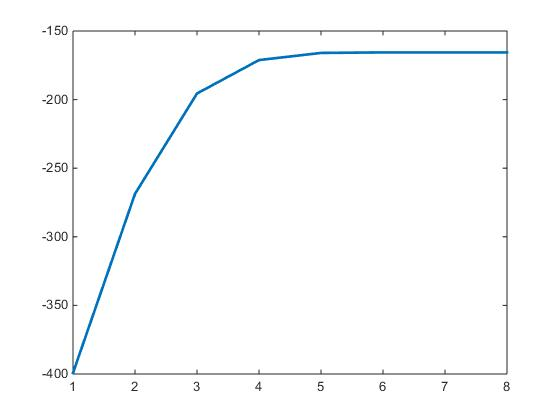
\includegraphics[scale=0.4]{images/ass1-img1.jpg}
\noindent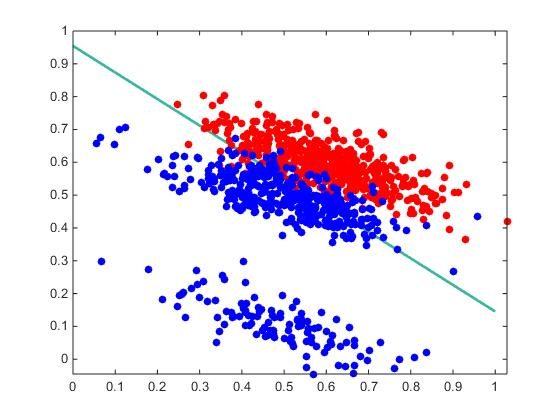
\includegraphics[scale=0.4]{images/ass1-img2.jpg}
\noindent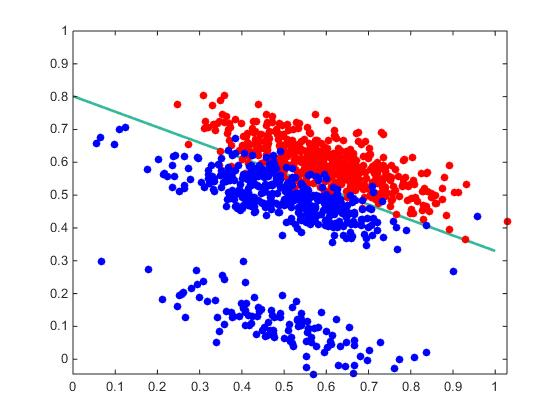
\includegraphics[scale=0.4]{images/ass1-img3.jpg}
\caption{Top-left: $C(w)$ as a function Newton-Raphson iteration; top-right: decision boundary for linear regression (already implemented); bottom: decision boundary for logistic regression}
\end{figure}

\medskip
We clearly see that the separator for logistic regression is better placed on the "fronteer" of the two types of data. The fact that the linear does worst here can be explained by the bunch of blue outliers at the bottom of the image.

\section{Logistic Regression and Regularization}

The regularization term in $C(w)$ results in an additional "$-2\lambda w$" term in the gradient calculus, and "$-2\lambda I$" in the Hessian calculus, where I is the identity matrix.
\\I added a parameter "lambda" in the functions "gradient.m" and "hessian.m" to take it into account. Twenty values of lambda are tested, logarithmically taken between 0.0001 and 100,  and ten cross-validations are made for each lambda.

We find an optimal lambda of 5,46. Here are the averaged losses for each lambda, and the decision boundary obtained on the test set :

\begin{figure}[!htbp]
\centering
\noindent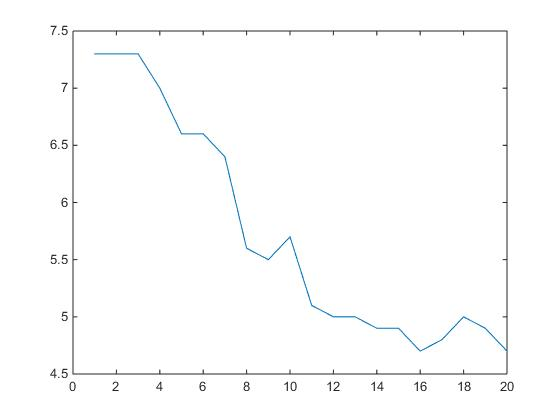
\includegraphics[scale=0.4]{images/ass1-img4.jpg}
\noindent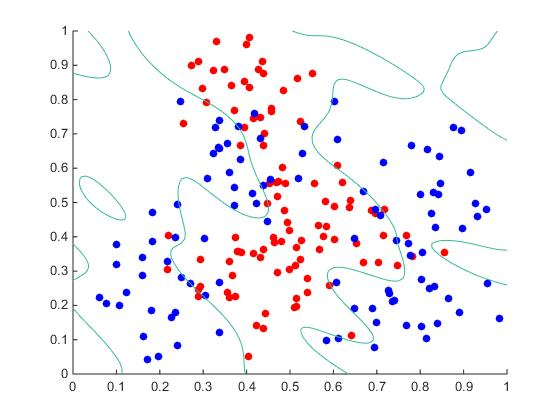
\includegraphics[scale=0.4]{images/ass1-img5.jpg}
\caption{Figure 2: Cross-validation error as a function of $\lambda$ and decision boundary for $\lambda^{*}$}
\end{figure}

On test set, we find 49 (24,5 \%) errors.
\\We here used a kernel method, to find the separator in higher dimension ($\mathbb{R}^{242}$ here), and then have it back in $\mathbb{R}^{2}$, this is why we have this form for the separator, and such a high number of errors that we cannot visualize.

To go further, we could try another method on the same train dataset (linear regression for example, just as in part "a"), do the same lambda selection and K-fold cross-validation procedure over it, and see which method gives the best results (i.e. the minimum number of errors on test dataset for instance).

\end{document}
